%
% Transportation Research Board conference paper template
% version 1.1
% 
% David R. Pritchard, http://davidpritchard.org
%   1.0 - Mar. 2009
%   1.1 - Sep. 2011, fixes for captions
%   2.0 - Mar. 2012, Reorganized title page incl. automatic counters

% PAGE LAYOUT
%------------------------------------------

% Custom paper settings...
\documentclass[titlepage,oneside,12pt]{article}

\oddsidemargin 0.0in
\topmargin -0.5in
\headheight 0.3in
\headsep 0.2in
\textwidth 6.5in
\textheight 9.0in
\setlength{\parindent}{0.5in}

% PAGE HEADER
%------------------------------------------
% Adjust the header text below (INSERT AUTHORS HERE)
\oddsidemargin 0.0in
\usepackage[tiny,rm]{titlesec}
\newpagestyle{trbstyle}{
	\sethead{Guilliard}{}{\thepage}
}
\pagestyle{trbstyle}

% HEADINGS
%------------------------------------------
\renewcommand*{\refname}{\uppercase{References}}
\titleformat{\section}{\bfseries}{}{0pt}{\uppercase}
\titlespacing*{\section}{0pt}{12pt}{*0}
\titleformat{\subsection}{\bfseries}{}{0pt}{}
\titlespacing*{\subsection}{0pt}{12pt}{*0}
\titleformat{\subsubsection}{\itshape}{}{0pt}{}
\titlespacing*{\subsubsection}{0pt}{12pt}{*0}

% LISTS
%------------------------------------------
% Adjust lists a little. Not quite perfectly fitting TRB style, but vaguely
% close at least.
\usepackage{enumitem}
\setlist[1]{labelindent=0.5in,leftmargin=*}
\setlist[2]{labelindent=0in,leftmargin=*}

% CAPTIONS
%------------------------------------------
% Get the captions right. Authors must still be careful to use "Title Case"
% for table captions, and "Sentence case." for figure captions.
\usepackage{ccaption}
\usepackage{amsmath}
\makeatletter
\renewcommand{\fnum@figure}{\textbf{FIGURE~\thefigure} }
\renewcommand{\fnum@table}{\textbf{TABLE~\thetable} }
\makeatother
\captiontitlefont{\bfseries \boldmath}
\captiondelim{\;}
%\precaption{\boldmath}


% CITATIONS
%------------------------------------------
% TRB uses an Author (num) citation style. I haven't found a way to make
% LaTeX/Bibtex do this automatically using the standard \cite macro, but
% this modified \trbcite macro does the trick.

% sort&compress option?
\usepackage[sort,numbers]{natbib}
	\newcommand{\trbcite}[1]{\citeauthor{#1} ({\it \citenum{#1}})}
\setcitestyle{round}


% LINE NUMBERING
%------------------------------------------
% TRB likes line numbers on drafts to help reviewers refer to parts of the
% document. The numbering is activated with the \linenumbers command immediately
% after \begin{document} You may need to install the lineno  package from CTAN.
\usepackage[pagewise,displaymath, mathlines]{lineno}
	\renewcommand\linenumberfont{\normalfont\small}


% COUNTERS
%------------------------------------------
% TRB requires the total number of words, figures, and tables to be displayed on
% the title page. This is possible under the totcount package on CTAN.
\usepackage{totcount}
	\regtotcounter{table} 	%count tables
	\regtotcounter{figure} 	%count figures

\newcommand\wordcount{
    \immediate\write18{texcount -sum -1 \jobname.tex > 'count.txt'} \input{count.txt} }

% FONTS
%------------------------------------------
% Times for text and math
%\usepackage{fontspec}
%\setmainfont{Times New Roman}
\usepackage{times} 
%\usepackage{mathptmx}
%\usepackage{newtxmath} 
%\DeclareMathAlphabet{\mathcal}{OMS}{cmsy}{m}{n}
% Some pdf conversion tricks? Unsure.
\usepackage[T1]{fontenc}
\usepackage{textcomp}
% Fonts will be broken by Sweave without this option
\usepackage[noae]{Sweave}


% OTHER PACKAGES
%------------------------------------------
% Add any additional \usepackage declarations here.

\usepackage{graphicx}
\usepackage{amssymb}
\usepackage{epstopdf}
\usepackage{color}
\usepackage{listings}
\usepackage{multicol}
\usepackage{subfigure}
\usepackage{tikz}
\usepackage{hyperref}
\usepackage{booktabs}
\usepackage{mathtools}
\usepackage{cleveref}
\DeclareGraphicsRule{.tif}{png}{.png}{`convert #1 `dirname #1`/`basename #1 .tif`.png}
\graphicspath{{plots/}}

\newcommand*\patchAmsMathEnvironmentForLineno[1]{%
  \expandafter\let\csname old#1\expandafter\endcsname\csname #1\endcsname
  \expandafter\let\csname oldend#1\expandafter\endcsname\csname end#1\endcsname
  \renewenvironment{#1}%
     {\linenomath\csname old#1\endcsname}%
     {\csname oldend#1\endcsname\endlinenomath}}% 
\newcommand*\patchBothAmsMathEnvironmentsForLineno[1]{%
  \patchAmsMathEnvironmentForLineno{#1}%
  \patchAmsMathEnvironmentForLineno{#1*}}%
\AtBeginDocument{%
\patchBothAmsMathEnvironmentsForLineno{equation}%
\patchBothAmsMathEnvironmentsForLineno{align}%
\patchBothAmsMathEnvironmentsForLineno{flalign}%
\patchBothAmsMathEnvironmentsForLineno{alignat}%
\patchBothAmsMathEnvironmentsForLineno{gather}%
\patchBothAmsMathEnvironmentsForLineno{multline}%
}

% TITLEPAGE
%-----------------------------------------
\begin{document}

	\linenumbers % comment out for final manuscript
	\thispagestyle{empty}

\begin{titlepage}
\begin{flushleft}

% Title
{\LARGE \bfseries A Non-homogenous Time Mixed Integer LP Formulation for Traffic Signal Control}\\[1cm]

Iain Guilliard \\
iguilliard@nicta.com.au\\[0.5cm]

%Gregory S. Macfarlane\\
%Georgia Institute of Technology \\
%790 Atlantic Drive \\
%Atlanta, GA 30332-0335 \\
%gregmacfarlane@gatech.edu\\[1cm]

\wordcount words + \total{figure} figures + \total{table} tables

\today
\end{flushleft}
\end{titlepage}


\newpage



\thispagestyle{empty}
\newcommand{\Net}{\mathcal{N}}
\newcommand{\Qset}{\mathcal{Q}}
\newcommand{\QPset}[1]{\mathcal{Q}_{#1}^{\mathcal{P}}}
\newcommand{\Lset}{\mathcal{L}}
\newcommand{\Pset}{\mathcal{P}}
\newcommand{\Fvec}[1]{\mathbf{F}_{#1}}
\newcommand{\Prvec}[1]{\mathbf{Pr}_{#1}}
\newcommand{\fvec}[1]{\mathbf{f}_{#1}}

% Uncomment for old style equations
%\newcommand*{\oldeq}{}

% Uncomment for new style equations with Lin and Wang subscripts
\newcommand*{\neweqsub}{}

% Uncomment for new in out flow variables
\newcommand*{\newinoutflow}{}

\ifdefined\oldeq
%
% Old style equations
%
\newcommand{\q}[2][n]{q_{#2}^{#1}}
\newcommand{\qin}[2][n]{q_{#2,in}^{#1}}
\newcommand{\qout}[2][n]{q_{#2,out}^{#1}}
\newcommand{\f}[3][n]{f_{#2,#3}^{#1}}
\newcommand{\inq}[2][n]{in_{#2}^{#1}}
\newcommand{\outq}[2][n]{out_{#2}^{#1}}
\newcommand{\p}[3][n]{p_{#2,#3}^{#1}}
\newcommand{\pd}[3][n]{d_{#2,#3}^{#1}}
\newcommand{\aph}[2][n]{\alpha_{#2}^{#1}}
\newcommand{\tn}[1][n]{t^{#1}}
\newcommand{\DT}[1][n]{\Delta t^{#1}}

\newcommand{\Nn}{\mathrm{N}}
\newcommand{\Qn}{|\mathcal{\Qset}|}
\newcommand{\Ln}{|\mathcal{\Lset}|}
\newcommand{\Pn}[1][\ell]{|\mathcal{\Pset}_{#1}|}
\newcommand{\TMAX}{T^{MAX}}
\newcommand{\QMAX}[1]{Q_{#1}^{MAX}}
\newcommand{\QIN}[1]{Q_{#1}^{IN}}
\newcommand{\QOUT}[1]{Q_{#1}^{OUT}}
\newcommand{\QDELAY}[1]{Q_{#1}^{DELAY}}
\newcommand{\FMAX}[2]{F_{#1,#2}^{MAX}}
\newcommand{\FTURN}[2]{F_{#1,#2}^{TURN}}
\newcommand{\PTMAX}[2]{PT_{#1,#2}^{MAX}}
\newcommand{\PTMIN}[2]{PT_{#1,#2}^{MIN}}
\newcommand{\CTMAX}[1]{CT_{#1}^{MAX}}
\newcommand{\CTMIN}[1]{CT_{#1}^{MIN}}

\else
\ifdefined\neweqsub
%
% New style equations subscript
%
\newcommand{\q}[2][n]{q_{#2,#1}}
\newcommand{\qin}[2][n]{q_{#2,#1}^{\mathrm{in}}}
\newcommand{\qout}[2][n]{q_{#2,#1}^{\mathrm{out}}}
\newcommand{\f}[3][n]{f_{#2\to#3,#1}}

%\ifdefined\newinoutflow
\newcommand{\inq}[2][n]{f_{in\to#2,#1}}
\newcommand{\outq}[2][n]{f_{#2\to out,#1}}
%\else
%\newcommand{\inq}[2][n]{in_{#2,#1}}
%\newcommand{\outq}[2][n]{out_{#2,#1}}
%\fi

\newcommand{\p}[3][n]{p_{#2,#3,#1}}
\newcommand{\pd}[3][n]{d_{#2,#3,#1}}
\newcommand{\aph}[2][n]{\alpha_{#2,#1}}
\newcommand{\tn}[1][n]{t_{#1}}
\newcommand{\DT}[1][n]{\Delta t_{#1}}

\newcommand{\Nn}{\mathrm{N}}
\newcommand{\Qn}{|\mathcal{\Qset}|}
\newcommand{\Ln}{|\mathcal{\Lset}|}
\newcommand{\Pn}[1][\ell]{|\mathcal{\Pset}_{#1}|}
\newcommand{\TMAX}{\mathrm{T}}
\newcommand{\QMAX}[1]{\mathrm{Q}_{#1}}

\ifdefined\newinoutflow
\newcommand{\QIN}[1]{\mathrm{F}_{in\to#1}}
\newcommand{\QOUT}[1]{\mathrm{F}_{#1\to out}}
\else
\newcommand{\QIN}[1]{\mathrm{Q}_{#1}^{\mathrm{in}}}
\newcommand{\QOUT}[1]{\mathrm{Q}_{#1}^{\mathrm{out}}}
\fi

\newcommand{\QDELAY}[1]{\mathrm{Q}_{#1}^{\mathrm{delay}}}
\newcommand{\FMAX}[2]{\mathrm{F}_{#1\to#2}}
\newcommand{\FTURN}[2]{\mathrm{Pr}_{#1\to#2}^{\mathrm{}}}
\newcommand{\PTMAX}[3][,]{\mathrm{\Phi}_{#2#1#3}^{\mathrm{max}}}
\newcommand{\PTMIN}[3][,]{\mathrm{\Phi}_{#2#1#3}^{\mathrm{min}}}
\newcommand{\CTMAX}[1]{\mathrm{\Psi}_{#1}^{\mathrm{max}}}
\newcommand{\CTMIN}[1]{\mathrm{\Psi}_{#1}^{\mathrm{min}}}



\else
%
% New style equations superscipt
%
\newcommand{\q}[2][n]{q_{#2}^{(#1)}}
\newcommand{\qin}[2][n]{q_{#2,in}^{(#1)}}
\newcommand{\qout}[2][n]{q_{#2,out}^{(#1)}}
\newcommand{\f}[3][n]{f_{#2\to#3}^{(#1)}}
\newcommand{\inq}[2][n]{in_{#2}^{(#1)}}
\newcommand{\outq}[2][n]{out_{#2}^{(#1)}}
\newcommand{\p}[3][n]{p_{#2,#3}^{(#1)}}
\newcommand{\pd}[3][n]{d_{#2,#3}^{(#1)}}
\newcommand{\aph}[2][n]{\alpha_{#2}^{(#1)}}
\newcommand{\tn}[1][n]{t^{(#1)}}
\newcommand{\DT}[1][n]{\Delta t^{(#1)}}

\newcommand{\Nn}{\mathrm{N}}
\newcommand{\Qn}{|\mathcal{\Qset}|}
\newcommand{\Ln}{|\mathcal{\Let}|}
\newcommand{\Pn}[1][\ell]{|\mathcal{\Pet}_{#1}|}
\newcommand{\TMAX}{\mathrm{T}}
\newcommand{\QMAX}[1]{\mathrm{Q}_{#1}}
\newcommand{\QIN}[1]{\mathrm{Q}_{#1}^{\mathrm{in}}}
\newcommand{\QOUT}[1]{\mathrm{Q}_{#1}^{\mathrm{out}}}
\newcommand{\QDELAY}[1]{\mathrm{Q}_{#1}^{\mathrm{delay}}}
\newcommand{\FMAX}[2]{\mathrm{F}_{#1\to#2}}
\newcommand{\FTURN}[2]{\mathrm{Pr}_{#1\to#2}^{\mathrm{}}}
\newcommand{\PTMAX}[3][,]{\mathrm{\Phi}_{#2#1#3}^{\mathrm{max}}}
\newcommand{\PTMIN}[3][,]{\mathrm{\Phi}_{#2#1#3}^{\mathrm{min}}}
\newcommand{\CTMAX}[1]{\mathrm{\Psi}_{#1}^{\mathrm{max}}}
\newcommand{\CTMIN}[1]{\mathrm{\Psi}_{#1}^{\mathrm{min}}}

\fi



%
% 
%

\section{Introduction}

{\bf Previous content:}

This report describes a new model for optimised traffic signal
planning using a MILP formulation. Previously,
\trbcite{lin2004enhanced} describe a MILP formulation for optimised
traffic signal planning based on the Cell Transmission Model of
\trbcite{daganzo1995cell}. However a CTM based model is limited in
scalability by the requirement that each road way in the network must
be partitioned up into segments that take exactly $\DT[]=1$ to
traverse at the free flow speed. We get around this limitation by
using a queue based model that supports non-homogeneous time steps,
and we will show how we can exploit this property to scale a network
without significant increase in the number of variables or loss of
quality.

{\bf Scott's suggested argument structure:}

\remark{I say we drop the issue of many segments and simply criticize
  the CTM by saying that it is not easy to make non-homogenous and
  that is what we need?  In general, the Intro probably has to push on
  the non-homogenous motivation a little earlier and forcefully since
  we're claiming *this* is the reason for the paper, the QTM and
  ultimately our evaluation comparing homogenous vs. non-homogenous.
  We may have broader (not fully validated) motivations but we need a
  watertight argument and paper.}

In practice, control of congested urban traffic networks ranges from
fixed time to actuated to adaptive (SCATS, SCOOT).  However there is
further opportunity to improve traffic scheduling through the use of
optimization techniques as proposed in various works
(Gartner, Lin and Wang, MARLIN -- Toronto, SURTRAC -- Smith).  In this
work, we specifically build on the MILP approach to traffic
optimization that extends previous work by Lin and Wang who
optimize traffic signals (discrete choices at each time step) in a 
Cell Transmission Model (CTM)~\trbcite{daganzo1995cell} of traffic flow.
Unfortunately a CTM based model is limited in
scalability by the requirement that each road way in the network must
be partitioned up into segments that take exactly $\DT[]=1$ to
traverse at the free flow speed.
This leads to a large number of cells
(and hence variables in the MILP) and it makes it difficult to
allow for variable length (non-homogenous) time steps in the model
updates that we demonstrate in this work
to be useful for optimized traffic signal planning over long horizons.

To allow for more parsimonious models of traffic flow and non-homogenous
time steps for updates, we introduce the queue transmission model (QTM) [succinct description needed], which offers the following
benefits:
\begin{itemize}
\item non-homogenous time steps which can keep the model compact over long horizons
\item models platoons without fine-grained cell-based road model or explicit variables to model platoons -- underlies a key precept in urban traffic control to let platoons pass through without stopping,
\item still leads to a MILP, albeit one with much fewer variables owing to the reduced number of queues vs. cells and the reduced number of time steps.
\end{itemize}
Some drawbacks -- does not capture nonlinear flow-density relationship of the
fundamental diagram.  \remark{Argue why this is OK for saturated
  urban networks at peak times.  Green waves in SCATS/SCOOT operate on
  principle of a fixed propagation time, so does Gartner's MILP model.
Captures the right level of detail without blowing up size of model.}

In the remainder of this paper, we show first how to formulate traffic flow
with fixed signals as an LP in the QTM; we then proceed to allow the
traffic signals to become discrete variables subject to optimization leading
to our final MILP formulation of traffic signal control.  We then experiment
with QTM-based control in a range of networks demonstrating the improved
scalability possible with non-homogeneous time steps in comparison to
the best homogenous time step and also the scalability of the model ---
we demonstrate near-optimal traffic control models over longer horizons and
larger networks than shown in previous implementations of MILP-based
traffic signal control.

\remark{Paper should follow the basic progression outlined above.  We
  could really use some pictures in the Intro to refer to here and
  subsequently -- both a traffic network divided into queues, and the
  concept of the piecewise linear evolution of traffic flow with
  non-homogenous time steps that I had provided in my early writeup.
  I think these help visually explain much of the context for the
  paper and its approach.}



\section{The Queue Transmission Model (QTM)}


%% TODO(fwt): We need to say that we handle expected number of cars instead of
%% physical cars, so its fine to have fractions of cars.

A Queue Transmission Model (QTM) is the tuple $(\Qset, \Lset, \vecDT, \MatQIN)$,
where \Qset and \Lset are, respectively, the set of queues and lights;
%
\vecDT is a vector of size \Nn representing the discretization of the problem
horizon $[0,\TMAX]$ and \authorHighlight{the duration in seconds of the $n$-th
time interval is denoted as \DT[n];}
%
%%
%% TODO(fwt): Maybe mention that car that are denied entry could be stored in a
%% infinity capacity queue and eventually be allowed to enter the network. Also
%% point out that this case doesn't happen in our experiments
%%
%% TODO(fwt): Maybe mention that add \QIN{i} can estimate through a model
%% learned from historical data.
%
and \MatQIN is a matrix $|\Qset| \times \TMAX$ in which \QIN{i}{n} represents
the flow of cars requesting to enter queue $i$ from the outside of the network
at time $n$.



A \textbf{traffic light} $\tl \in \Lset$ is defined as the tuple~$(\CTMIN{\tl},
\CTMAX{\tl}, \Pset_\tl, \VecPTMIN{\tl}, \VecPTMAX{\tl})$, where:
%
\begin{itemize*}[label={}]
%
\item $\Pset_\tl$ is the set of phases of $\tl$;
%
\item \CTMIN{\tl} (\CTMAX{\tl}) is the minimum (maximum) allowed cycle time for
\tl; and
%
\item \VecPTMIN{\tl} (\VecPTMAX{\tl}) is a vector of size $|\Pset_\tl|$ and
  \PTMIN{\tl}{k} (\PTMAX{\tl}{k}) is the minimum (maximum) allowed time for
  phase $k \in \Pset_\tl$. 
%
\end{itemize*}


A \textbf{queue} $i \in \Qset$ represents a segment of road that vehicles
traverse at free flow speed; once traversed, the vehicles are vertically stacked
in a stop line queue.
% of maximum capacity \QMAX{i}.
%
Formally, a queue~$i$ is defined by the tuple~$(\QMAX{i}, \QDELAY{i}, \QOUT{i},
\Fvec_i, \Prvec_i, \QPset{i})$ where:
%
\begin{itemize*}[label={}]
%
%% TODO(fwt): clarify that this is the capacity of stop line queue
\item \QMAX{i} is the maximum capacity of $i$;
%
\item \QDELAY{i} is the time required to traverse $i$ and reach the stop line;
%
\item \QOUT{i} represents the maximum traffic flow from $i$ to the outside of
  the modeled network;
%
\item $\Fvec_i$ and $\Prvec_i$ are vectors of size \Qn and their $j$-th entry
  (i.e., \FMAX{i}{j} and \FTURN{i}{j}) represent the maximum flow from queue $i$
  to $j$ and the turn probability from $i$ to $j$ ($\sum_{j \in
  \Qset}\FTURN{i}{j} = 1$), respectively; and
%
\item \QPset{i} denotes the set of traffic light phases controlling the outflow
  of queue $i$.
%
\end{itemize*}


Differently than the CTM \cite{daganzo1994cell,lin2004enhanced}, the
\authorHighlight{QTM does not assume that $\DT[n] = \QDELAY{i}$ for all $n$,
that is, the QTM can represent non-homogeneous time intervals.
%
%%(\cref{subfig:example}).
%
The only requirement over \DT[n] is that no traffic light maximum phase time is
smaller than any \DT[n] since phase changes occur only between time intervals;
formally, $\DT[n] \le \min_{\tl \in \Lset, k \in \Pset_\tl} \PTMAX{\tl}{k}$ for
all $n \in \{1,\dots,\Nn\}$.}
%
% TODO \toIain{Maybe bring forward a small network and any other figure that
% would help illustrate the model and comment about it.}



\subsection{Computing Traffic Flows with QTM}

In this section, we present how to compute traffic flows using QTM and
\authorHighlight{non-homogeneous time intervals \DT[]}.
%
We assume for the remainder of this section that a \emph{valid} control plan for
all traffic lights is fixed and given as parameter;
%
formally, for all $\tl \in \Lset$, $k \in \Pset_\tl$, and interval $n \in
\{1,\dots,N\}$, the binary variable $\p{\tl}{k}$ is known a priori and indicates
if phase $k$ of light \tl is active~(i.e., $\p{\tl}{k} = 1$) or not on interval
$n$.


We represent the problem of finding the maximal flow between
capacity-constrained queues as a Linear Program~(LP) over the following
variables defined for all interval $n \in \{1,\dots,\Nn\}$ and queues $i$ and
$j$:
%
\begin{itemize*}[label={}]
%
\item $\q{i} \in [0,\QMAX{i}]$: traffic volume waiting in the stop line of queue
  $i$ at the beginning of interval~$n$;
%
\item $\inq{i} \in [0,\QIN{i}{n}]$: inflow to the network via queue $i$ during
  interval $n$;
%
\item $\outq{i} \in [0,\QOUT{i}]$: outflow from the network via queue $i$ during
  interval $n$; and
%
\item $\f{i}{j} \in [0,\FMAX{i}{j}]$: flow from queue $i$ into queue $j$ during
  interval $n$.
%
\end{itemize*}



%% FWT: These constraints are not necessary because we defined the domain of the
%% variables in the paragraph above
%\inq{i} &\le \QIN{i}{n} \tag{C1}\label{eq:C1}\\ 
%\outq{i} &\le \QOUT{i} \tag{C2}\label{eq:C2}\\
% \q{i} &\le \QMAX{i} \tag{C9}\label{eq:C9}\\




The maximum traffic flow from queue $i$ to queue $j$ is enforced by
\cref{c:turnProbAndMaxFlow}.
%
The inner inequality of \eqref{c:turnProbAndMaxFlow} ensures that only the
fraction $\FTURN{i}{j}$ of the total internal outflow of $i$ goes to $j$, and
the outer inequality forces the flow from $i$ to $j$ to be zero if all phases
controlling $i$ are inactive (i.e., $\p{\ell}{k} = 0$ for all $k \in
\QPset{i}$).
%
%If more than one phase $\p{\ell}{k}$ is active, then
%\eqref{c:turnProbAndMaxFlow} is subsumed by the domain upper bound of
%$\f{i}{j}$.
%
\begin{cAlign} 
%
\f{i}{j} \le \FTURN{i}{j} \sum_{k=1}^{\Qn} \f{i}{k}
%\tagconstrain{c:turnProb}\\ \f{i}{j}
\le \FMAX{i}{j} \sum_{\p{\ell}{k} \in \QPset{i}} {\p{\ell}{k}}
%\tagconstrain{c:maxFlow}
\tagconstrain{c:turnProbAndMaxFlow}
%
\end{cAlign}




%% TODO(fwt): improve the beginning of this paragraph

To simplify the presentation of remainder of the LP, we define the helper
variables \qin{i}~\eqref{def:qin} and \qout{i}~\eqref{def:qout} to,
respectively, represent the volume of traffic to enter and leave queue $i$
during interval~$n$, and  $\tn[n] = \sum_{x=1}^{n} \DT[x]$ to represent the time
elapsed since the beginning of the problem until the end of interval \DT[n].
%
%
%\tn[n]~\eqref{def:tn}
%
%
\begin{cAlign}
%
\qin{i} &= \DT (\inq{i} + \textstyle \sum_{j=1}^{\Qn} \f{j}{i}) \tagconstrain{def:qin} \\
%
\qout{i} &= \DT (\outq{i} + \textstyle  \sum_{j=1}^{\Qn} \f{i}{j})
\tagconstrain{def:qout}
%\\
%
%\tn[n] &= \sum_{x=1}^{n} \DT[x] \tagconstrain{def:tn}
%
\end{cAlign}



% Introduce the idea of V_i
\authorHighlight{In order to account for the misalignment of the different \DT[]
and \QDELAY{i}, we need to find the volume of traffic that entered queue $i$
between two arbitrary points in time $x$ and $y$ ($x \in [0,\TMAX]$, $y \in
[0,\TMAX]$, and $x < y$), i.e., $x$ and $y$ might not coincide with any $t_n$
for $n \in \{1,\dots,N\}$.
%
This volume of traffic, denoted as $\Vol_i(x,y)$, is obtained by integrating
\qin{i} over $[x,y]$ and is defined in~\eqref{eq:vol} where $m$ and $w$ are the
index of the time intervals s.t. $\tn[m] \le x < \tn[m+1]$ and $\tn[w] \le y <
\tn[w+1]$.
%
Because the QTM dynamics are \emph{piecewise linear}, \qin{i} is a step function
w.r.t.~time and this integral reduces to the sum of \qin{i} over the intervals
contained in $[x,y]$ and the appropriate fraction of \qin[m]{i} and \qin[w]{i}
representing the misaligned beginning and end of $[x,y]$.
%
{\small
\begin{equation}
\Vol_{i}(x,y)\! =\!
  (\tn[m+1]\!-\! x) \frac{\qin[m]{i}}{\DT[m]}\!+\!\left(
  \sum_{k=m+1}^{w-1} \qin[k]{i} \right)\!+\! (y\!-\! \tn[w])
  \frac{\qin[w]{i}}{\DT[w]}
  \label{eq:vol}
\end{equation}}
}


Using these helper variables, \eqref{c:qUpdate} represents the flow conservation
principle for queue $i$ where $\Vol_i(\tn[n-1]-\QDELAY{i},\tn[n]-\QDELAY{i})$ is
the volume of cars that reached the stop line during \DT[n].
%
Since \vecDT and \QDELAY{i} for all queues are known a priori, the indexes $m$
and $w$ used by $V_i$ can be pre-computed in order to encode \eqref{eq:vol};
moreover, \eqref{c:qUpdate} represents a non-first order Markovian update
because the update considers the previous $w-m$ time steps.
%
To ensure that the total volume of traffic traversing $i$ (i.e.,
$\Vol_i(\tn[n] - \QDELAY{i}, \tn[n])$) and waiting at the stop line does not
exceed the capacity of the queue, we apply~\eqref{c:10}.
%
\begin{cAlign}
%
& \q{i} = \q[n\!-\!1]{i} \! - \! \qout[n\!-\!1]{i} \! + \!
\Vol_i(\tn[n\!-\!1] \! - \! \QDELAY{i},\tn[n] \! - \! \QDELAY{i}) \tagconstrain{c:qUpdate}\\
%
& \Vol_i(\tn[n] - \QDELAY{i}, \tn[n]) + \q{i} \le \QMAX{i}
\tagconstrain{c:10}
%
\end{cAlign}


%\begin{figure*}[t!]
%\centering
%%  trim={<left> <lower> <right> <upper>}
%\includegraphics[width=1.0\textwidth,trim={0cm 0cm 0cm 0cm},clip]{convergence_NH.pdf}
%\caption{An example showing the convergence between a homogeneous solution with
%$\Delta t=1.0$ and a non-homogeneous solution over 30 seconds for the same
%network. By using non-homogeneous time steps the same solution is found with
%only 14 sample points compared to 30 for homogeneous solution.}
%\label{fig:converg_c}
%\end{figure*}



As with MILP formulations of CTM (e.g. \trbcite{lin2004enhanced}),
QTM is also susceptible to \emph{withholding traffic}, i.e., the
optimizer might prevent cars from moving from $i$ to $j$ even though the
associated traffic phase is active and $j$ is not full, e.g., this may
reserve space for traffic from an alternate approach that allows the MILP
to minimize delay in the long-term even though it leads to unintuitive traffic
flow behavior.
%
We address this well-known issue through our objective function~\eqref{eq:objFunc} by
maximizing the total outflow~\qout{i}
%
%(i.e., both internal and external outflow)
%
of~$i$ plus the inflow~\inq{i} from the outside of the network to~$i$.
%
This quantity is weighted by the remaining time until the end of the problem
horizon \TMAX to force the optimizer to allow as much traffic volume as possible
into the network and move traffic to the outside of the network as soon as
possible.
%% FWT: not sure if we need to give this extra details
%\trbcite{lin2004enhanced} derive an objective function for the minimisation of
%total delay based on the difference between the cumulative departure and
%arrival curves at the origin and destination. However, such an approach
%requires the network to be cleared at the end of the optimisation period.


\begin{equation}
\max 
 \sum_{n=1}^{\Nn} \sum_{i=1}^{\Qn} (\TMAX - \tn + 1) (\qout{i} + \inq{i})
\tag{O1}\label{eq:objFunc}
\end{equation}


%\begin{figure*}[t!]
%\centering
%%  trim={<left> <lower> <right> <upper>}
%\includegraphics[width=0.55\textwidth,trim={0cm 0cm 0cm 0cm},clip]{cumu_plot_final_6l.pdf}
%\caption{Cumulative arrival (blue) and departure (green) curves, and the
%resulting delay curve (red). The departure curve is maximized by the objective
%function \eqref{eq:objFunc}, which has the same effect as minimizing the area
%under the delay curve.}
%\label{fig:cumu_delay_plot}
%\end{figure*}


The objective \eqref{eq:objFunc} corresponds to minimizing delay in CTM models,
e.g., \eqref{eq:objFunc} is equivalent to the objective function (O3) in
\trbcite{lin2004enhanced} for their parameters $\alpha = \beta = 1$.
%
%
%Figure (fig:cumu-delay-plot) depicts this equivalence using the cumulative
%number of cars entering and leaving a network as a function of time.
%%
%The delay experienced by the vehicles travelling through this network (red curve
%in Figure (fig-cumu-delay-plot) equals the horizontal difference at each point
%between the cumulative departure and arrival curves (less the free flow travel
%time through the network).
%%
%Maximizing \qout{i} weighted by $(\TMAX - \tn +1)$ in \eqref{eq:objFunc} is the
%same as forcing the departure curve to be as close as possible to the arrival
%curve as early as possible; therefore, the area between arrival and departure is
%minimized, which in turn minimizes the delay.



%The objective function~\eqref{eq:objFunc} and
%constraints~(\ref{c:turnProb}--\ref{c:10}) form the LP representing the
%dynamic, piecewise linear model of flow in a QTM network over time when a
%control plan \p{\tl}{k} is given as an input parameter.



%\begin{figure*}[t!]
%\centering
%\subfigure[]{
%\label{subfig:converg_a}
%\includegraphics[width=1.0\textwidth,trim={0cm 0cm 0cm 0cm},clip]{convergence.pdf}
%}
%\subfigure[]{
%\label{subfig:converg_b}
%\includegraphics[width=1.0\textwidth,trim={0cm 0cm 0cm 0cm},clip]{convergence_vari.pdf}
%}
%\label{fig:conv}
%%
%\caption{Approximations of a queue volume obtained using homogeneous
%\DT[] = 1s using: (a) homogeneous \DT[] = 2.5s and 5s; and (b) non-homogeneous
%$\DT[n] \approx 0.0956n + 0.9044$ for $n \in \{1,\dots,17\}$.  Here we see
%that (b) achieves accuracy in the near-term that somewhat degrades over
%the long-term, where accuracy will be less critical for receding horizon control.}
%%% Note: would actually be nice to say something about
%%
%\end{figure*}


%To illustrate the representation tradeoff offered by non-homogeneous time
%intervals, we computed flows and queue volumes for a fixed signal control plan
%derived for homogeneous \mbox{\DT[n] = 1s} (ground truth) using different
%discretizations.
%%
%Figure (subfig:converg-a) shows the approximation of the ground truth using
%homogeneous \DT[] = 2.5 and \DT[] = 5.0, and Figure (subfig:converg-b) using
%non-homogeneous time intervals that linearly increases from 1s to 2.5s, i.e.,
%$\DT[n] \approx 0.0956n + 0.9044$ for $n \in \{1,\dots,17\}$.
%%
%As Figure (subfig:converg-a) shows, large time steps can be rough approximations
%of the ground truth.
%%
%Non-homogeneous discretization (Figure (subfig:converg-b)) exploit this fact to
%provide a good approximation in the initial time steps and progressively
%decrease precision for points far in the future.



\section{Traffic Control with MILP-encoded QTM}

In this section, we show how to compute the optimal control plan by extending
the LP (\ref{eq:objFunc},~\ref{c:turnProbAndMaxFlow}--\ref{c:10}) into an
Mixed-Integer LP (MILP).
%
Formally, for all~$\tl \in \Lset$, $k \in \Pset_\tl$, and interval $n \in
\{1,\dots,N\}$, the phase activation parameter~$\p{\tl}{k} \in \{0,1\}$ becomes
a free variable to be optimized.
%
In order to obtain a valid control plan, we enforce that one phase of traffic
light \tl is always active at any interval~$n$~\eqref{c:onlyOnePhaseOn} and that
phase changes happen sequentially~\eqref{c:seqPhases}
%
%, i.e., if phase~$k$ was
%active during interval~$n-1$ and has become inactive in interval~$n$, then
%phase~$k+1$ must be active in interval~$n$.
%
(\eqref{c:seqPhases} assumes that $k+1$ equals 1 if $k = \Pn{}$).
%
%% TODO: We need to understand this issue better:
% \toIain{I removed the constraint $\p{\ell}{k} + \p{\ell}{k+1} \le 1$ because it
% is subsumed by $\p{\ell}{k} \in \{0,1\}$ and \eqref{c:onlyOnePhaseOn}}
%
%
%% FWT: note sure if the text bellow is necessary
%Note that there could be more than one queue mapped to each $\p[]{\ell}{k}$, or
%their could be none
%
\begin{cAlign}
%
\textstyle \sum_{k=1}^{\Pn} \p{\ell}{k} &= 1\tagconstrain{c:onlyOnePhaseOn}\\
%
\p[n-1]{\ell}{k} &\le \p{\ell}{k} + \p{\ell}{k+1}\tagconstrain{c:seqPhases}
%
\end{cAlign}


%\begin{figure*}[t!]
%\centering
%%  trim={<left> <lower> <right> <upper>}
%\subfigure[]{
%\label{fig:pd:inc}
%\includegraphics[width=0.45\textwidth]{phase_plot_fig_1.pdf}}
%\subfigure[]{
%\label{fig:pd:inactive}
%\includegraphics[width=0.45\textwidth]{phase_plot_fig_2.pdf}}
%\subfigure[]{
%\label{fig:pd:resetAndLB}
%\includegraphics[width=0.45\textwidth]{phase_plot_fig_3.pdf}}
%\subfigure[]{
%\label{fig:cycleTimeC}
%\includegraphics[width=0.45\textwidth]{phase_plot_fig_4.pdf}}
%%
%\caption{Visualization of constraints (\ref{c:pd:incUB}--\ref{c:cycleUB})
%for a traffic light \tl as a function of time.
%%
%(a--c) present, pairwise, the constraints (\ref{c:pd:incUB}--\ref{c:minPhase})
%for phase $k$ (\pd{\ell}{k} as the black line) and the activation variable
%\p[n]{\ell}{k} in the small plot.
%%
%(d) presents the constraints for the cycle time of \tl (\ref{c:cycleLB} and
%\ref{c:cycleUB}), where T.C.T. is the total cycle time and is the left hand side
%of both constraints.
%%
%For this example, $\PTMIN{\ell}{k}=1$, $\PTMAX{\ell}{k}=3$, $\CTMIN{\ell}=7$, and
%$\CTMAX{\ell}=8$.}
%\label{fig:phase_plots}
%\end{figure*}



Next, we enforce the minimum and maximum phase durations (i.e.,
$\PTMIN{\ell}{k}$ and $\PTMAX{\ell}{k}$) for each phase $k \in \Pset_\tl$ of
traffic light \tl.
%
To encode these constraints, we use the helper variable $\pd{\ell}{k} \in
[0,\PTMAX{\ell}{k}]$, defined by constraints
(\ref{c:pd:incUB}--\ref{c:pd:reset}), that:
%
(i) holds the elapsed time since the start of phase $k$ when $\p[n]{\ell}{k}$ is
active~(\ref{c:pd:incUB},\ref{c:pd:incLB});
%
(ii) is constant and holds the duration of the last phase until the next
activation when $\p[n]{\ell}{k}$ is
inactive~(\ref{c:pd:inactiveUB},\ref{c:pd:inactiveLB}); and
%
(iii) is restarted when phase~$k$ changes from inactive to
active~\eqref{c:pd:reset}.
%
Notice that (\ref{c:pd:incUB}--\ref{c:pd:reset}) employs the \textit{big-M}
method to turn the cases that should not be active into subsumed constraints
based on the value of $\p[n]{\tl}{k}$.
%
We use~\PTMAX{\ell}{k} as our large constant since $\pd[n]{\ell}{k} \le
\PTMAX{\ell}{k}$ and $\DT[n] \le \PTMAX{\ell}{k}$.
%
Similarly, \cref{c:minPhase} ensures the minimum phase time of $k$ and is
not enforced while $k$ is still active.
%
%Figures (fig:pd:inc,fig:pd:inactive,fig:pd:resetAndLB) present an example of how
%(\ref{c:pd:incUB}--\ref{c:minPhase}) work together as a function of the time $n$ 
%for $\pd[n]{\ell}{k}$; the domain constraint $0 \le \pd[n]{\ell}{k} \le
%\PTMAX{\ell}{k}$ for all $n \in \{1,\dots,\Nn\}$ is omitted for clarity.
%
%% FWT: I think the mathematical definition of \pd is redundant now.
%\begin{equation}
%\pd{\ell}{k} = 
%\begin{cases}
%\pd[n-1]{\ell}{k} + \DT[n-1] & \p[n-1]{\ell}{k}=1,\p{\ell}{k}=1\\
%\pd[n-1]{\ell}{k} & \p{\ell}{k}=0\\
%0 & \p[n-1]{\ell}{k}=0,\p{\ell}{k}=1
%\end{cases}
%\label{def:pd}
%\end{equation}
%
%% TODO(fwt): I believe that that \pd{\ell}{k} (above) could be redefined by
%% shifting it by delta_n resulting in a d_{l,k,n} representing the total time
%% until the end of interval **n** instead of n-1. This would be more intuitive
%% and would simplify c:cycleLB and c:cycleUB. This is what I propose:
%% d_{l,k,n} = d_{l,k,n-1} + delta-t_{n}  if p_{l,k,n-1} = p_{l,k,n} = 1
%%           = d_{l,k,n-1}                if p_{l,k,n} = 0
%%           = delta-t_{n}                if p_{l,k,n-1} 0 and p_{l,k,n} = 1
%
%% FWT: this constraint is define as the variable domain
%\pd{\ell}{k} &\le \PTMAX{\ell}{k}\tag{C19}\label{eq:C19}\\
%
\begin{cAlign}
%
\pd{\ell}{k} &\le
  \pd[n-1]{\ell}{k} + \DT[n-1] \p[n-1]{\ell}{k} 
  + \PTMAX{\ell}{k} (1 - \p[n-1]{\ell}{k})\tagconstrain{c:pd:incUB}\\
%
\pd{\ell}{k} &\ge
  \pd[n-1]{\ell}{k} + \DT[n-1] \p[n-1]{\ell}{k}
  - \PTMAX{\ell}{k} (1 - \p[n-1]{\ell}{k})\tagconstrain{c:pd:incLB}\\
%
\pd{\ell}{k} &\le \pd[n-1]{\ell}{k} + \PTMAX{\ell}{k} \p[n-1]{\ell}{k}
  \tagconstrain{c:pd:inactiveUB}\\
\pd{\ell}{k} &\ge \pd[n-1]{\ell}{k} - \PTMAX{\ell}{k} \p{\ell}{k}
  \tagconstrain{c:pd:inactiveLB}\\
%\end{cAlign}
%%
%\begin{cAlign}
%%
\pd{\ell}{k} &\le \PTMAX{\ell}{k}(1 - \p{\ell}{k} + \p[n-1]{\ell}{k})
  \tagconstrain{c:pd:reset}\\
%
\pd{\ell}{k} &\ge \PTMIN{\ell}{k}(1 - \p{\ell}{k}) \tagconstrain{c:minPhase}
%
\end{cAlign}
%


Lastly, we constrain the sum of all the phase durations for light \tl to be
within the cycle time limits \CTMIN{\tl}~\eqref{c:cycleLB} and
\CTMAX{\tl}~\eqref{c:cycleUB}.
%
In both \eqref{c:cycleLB} and \eqref{c:cycleUB}, we use the duration of phase 1
of \tl from the previous interval $n-1$ instead of the current interval $n$
because \eqref{c:pd:reset} forces \pd[n]{\tl}{1} to be 0 at the beginning of
each cycle;
%
however, from the previous end of phase 1 until $n-1$, \pd[n-1]{\tl}{1} holds
the correct elapse time of phase 1.
%
Additionally, \eqref{c:cycleLB} is enforced right after the end of the each
cycle, i.e., when its first phase is changed from inactive to active.
%
%%The value \eqref{c:cycleLB} and \eqref{c:cycleUB} over time for a traffic light
%%\tl is illustrated in Figure (fig:cycleTimeC).
%
\begin{cAlign}
%
\pd[n-1]{\ell}{1} + \sum\limits_{k=2}^{\Pn} \pd{\ell}{k} &\ge \CTMIN{\ell}
(\p{k}{1} - \p[n-1]{k}{1}) \tagconstrain{c:cycleLB}\\
%
\pd[n-1]{\ell}{1} + \sum\limits_{k=2}^{\Pn} \pd{\ell}{k} &\le \CTMAX{\ell}
\tagconstrain{c:cycleUB}
%
\end{cAlign}
%
The MILP~(\ref{eq:objFunc},~\ref{c:turnProbAndMaxFlow}--\ref{c:cycleUB}) encodes
the problem of finding the optimal traffic control plan in a QTM network without
light rail.

\paragraph{Light Rail Constraints}
%
To incorporate a fixed-schedule light rail in our model, we post-process our
MILP model by fixing the free variable $\p[n]{\tl}{k}$ for all $n$ s.t.\ the
light rail uses phase $k$ of \tl at time $n$.
%
Formally, given a schedule $S_{\tl}(k,n) \in \{0,1\}$ where~$1$ represents that
the light rail uses phase $k$ of \tl at time $n$, we replace
(\ref{c:pd:incUB}--\ref{c:minPhase}) by \eqref{c:forceTransit} and
\eqref{c:pd:holdTransit} when $\sum_{k} S_{\tl}(k,n) > 0$.
%
\begin{cAlign}
%
\p[n]{\ell}{k} &= S_{\ell}(k,n)\tagconstrain{c:forceTransit}\\
%
\pd{\ell}{k} &= \pd[n-1]{\ell}{k}\tagconstrain{c:pd:holdTransit}
%
\end{cAlign}


%To incorporate a fixed-schedule light rail in our model, we enforce phase $k$ used
%by the light rail is always on when the transit crosses at light \tl, i.e., we add
%the constraint $\p[n]{\ell}{k} = 1$ for all $n$ s.t.\ the light rail uses phase $k$
%of \tl at time $n$.
%%
%%
%We also hold $\pd{\ell}{k}$ constant while the light rail crosses \tl, i.e., 
%$\pd{\ell}{k} = \pd[n-1]{\ell}{k}$.
%%
%Since the light rail schedule is fixed and known a priori, adding these extra
%constraints are done in a preprocessing phase before the MILP is solved.


\section{Empirical Evaluation}
  
In this section we compare the solutions for traffic networks modeled as a QTM
using homogeneous and non-homogeneous time intervals w.r.t.\ to two evaluation criteria:
%
the quality of the solution and convergence to the optimal solution vs.\ the number
of time steps.
%
% TODO \fnremark{FWT: I don't think that optimal is the best word here since
%we arbitrarily fixed a value of \DT[]. Also, there is the technical problem that
%Gurobi might not have found the true optimal.}
%
Specifically, we compare the quality of solutions based on the total travel time and we also
consider the third quartile and maximum of the observed delay distribution.
%
%% TODO(fwt): maybe define what we mean by optimal here, for instance
%
%For our experiments, we consider as optimal solution, the MILP solution of a
%QTM using small enough homogeneous \DT[] with unlimited computational
%resources.
%
\revinout{The hypothesis we wish to evaluate in this paper are}{Our hypotheses are}{2.5}:
%
(i) the quality of the non-homogeneous solutions is at least as good as the
homogeneous ones when the number of time intervals~\Nn is fixed; and 
%
(ii) the non-homogeneous approach requires less time intervals (i.e., smaller
\Nn) than the homogeneous approach to converge to the optimal solution.
%
In the remainder of this section, we present the traffic networks considered in
the experiments, our methodology, and the results.



\subsection{Networks}



\begin{figure*}[t!]
\centering
%  trim={<left> <lower> <right> <upper>}
\subfigure[]{
\label{subfig:network1}
\includegraphics[width=0.45\textwidth]{network_1.pdf}}
\subfigure[]{
\label{subfig:network2}
\includegraphics[width=0.45\textwidth]{network_2.pdf}}
\subfigure[]{
\label{subfig:network3}
\includegraphics[width=0.45\textwidth]{network_3.pdf}}
\subfigure[]{
\label{subfig:demand_plot}
\includegraphics[width=0.45\textwidth]{demand_plot.pdf}}
\caption{(a--c) Networks used to evaluate the QTM performance.
%
(d) Demand profile of the queues marked as \qLowTraf,
\qHighTraf, and \qVarTraf for our experiments.}
\label{fig:networks}
\end{figure*}



We consider three networks of increasing complexity (\cref{fig:networks}): an
avenue crossed by three side streets; a 2-by-3 grid; and a 3-by-3 grid with a
diagonal avenue.
%
The queues receiving cars from outside of the network are marked in
\cref{fig:networks} and we refer to them as input queues.
%
The maximum queue capacity~(\QMAX{i}) is 60 cars for non-input queues and
infinity for input queues to prevent interruption of the input demand due to
spill back from the stop line. 
%
The traversal time of each queue $i$~(\QDELAY{i}) is set at 9s (a distance of
125m with a free flow speed of 50km/h).
%
For each street, flows are defined from the head of each queue $i$ into the tail of the next
queue $j$;
%
there is no turning traffic ($\FTURN{i}{j}=1$), and the maximum flow rate
between queues, \FMAX{i}{j}, is set at 5 cars/s.
%
All traffic lights have two phases, north-south and east-west, and lights 2, 4
and 6 of network 3 have the additional northeast-southwest phase to control the
diagonal avenue.
%
For networks 1 and 2, \PTMIN{\tl}{k} is 1s, \PTMAX{\tl}{k} is 3s, \CTMIN{\tl} is
2s, and \CTMAX{\tl} is 6s, for all traffic light \tl and phase $k$.
%
For network 3, \PTMIN{\tl}{k} is 1s and \PTMAX{\tl}{k} is 6s for all \tl and
$k$; and \CTMIN{\tl} is 2s and \CTMAX{\tl} is 12s for all lights \tl except for
lights 2, 4 and 6 (i.e., lights also used by the diagonal avenue) in which
\CTMIN{\tl} is 3s and \CTMAX{\tl} is 18s.




\subsection{Experimental Methodology}

%\begin{table}[h]
%\caption{Network Demand Profiles (vehicles per second)}
%\label{tab:network_demand}
%\centering
%\begin{tabular}{cccccc}
%\toprule
%& Inflow Queues & 0 - 55 s & 55 - 70 s & 70 - 85 s & > 85 s\\
%\midrule
%\multirow{2}{*}{Network 1}&$q_0$ & 1 & 1 & 1 & 0 \\
%&$q_4, q_7$ & 4 & 4 & 4 & 0 \\
%&$q_1,q_{10}$& 2 & 4 & 2 & 0 \\
%\midrule
%\multirow{2}{*}{Network 2}&$q_0$ & 1 & 1 & 1 & 0 \\
%&$q_4,q_7,q_{14}$& 4 & 4 & 4 & 0 \\
%&$q_1, q_{10},q_{18}$ & 2 & 4 & 2 & 0 \\
%\midrule
%\multirow{2}{*}{Network 3}&$q_0$ & 1 & 1 & 1 & 0 \\
%&$q_4,q_7,q_{14},q_{25},$& 4 & 4 & 4 & 0 \\
%&$q_1, q_{10},q_{18},q_{29},q_{36},q_{40},q_{44}$ & 2 & 4 & 2 & 0 \\
%\bottomrule\\
%\end{tabular}
%\end{table}


For each network, a constant background level traffic is injected in the network
in the first 55s to allow the solver to settle on a stable policy.
%
Then a spike in demand is introduced in the queues marked as \qVarTraf
(\cref{fig:networks}) from time 55s to 70s to trigger a policy change.
%
%with the expectation that plans generated with longer look ahead will produce a
%more coordinated global policy change.
%
From time 70s to 85s, the demand is returned to the background level, and then
reduced to zero for all input queues.
%
We extend the problem horizon~\TMAX until all cars have left the network.
%
By clearing the network, we can easily measure the total travel time for all the
traffic as the area between the cumulative arrival and departure curves measured
at the boundaries of the network.
%
%TODO \fnremark{FWT: is this explanation of how to compute the total travel time
%still necessary?}
%
%\cref{tab:network_demand} presents the demand profile of each network.
%
The background level for the input queues are 1, 4 and 2 cars/s for queues
marked as \qLowTraf, \qHighTraf and \qVarTraf (\cref{subfig:demand_plot}),
respectively; and during the high demand period, the queues \qVarTraf receive 4
cars/s.




\begin{figure*}[t!]
\centering
%  trim={<left> <lower> <right> <upper>}
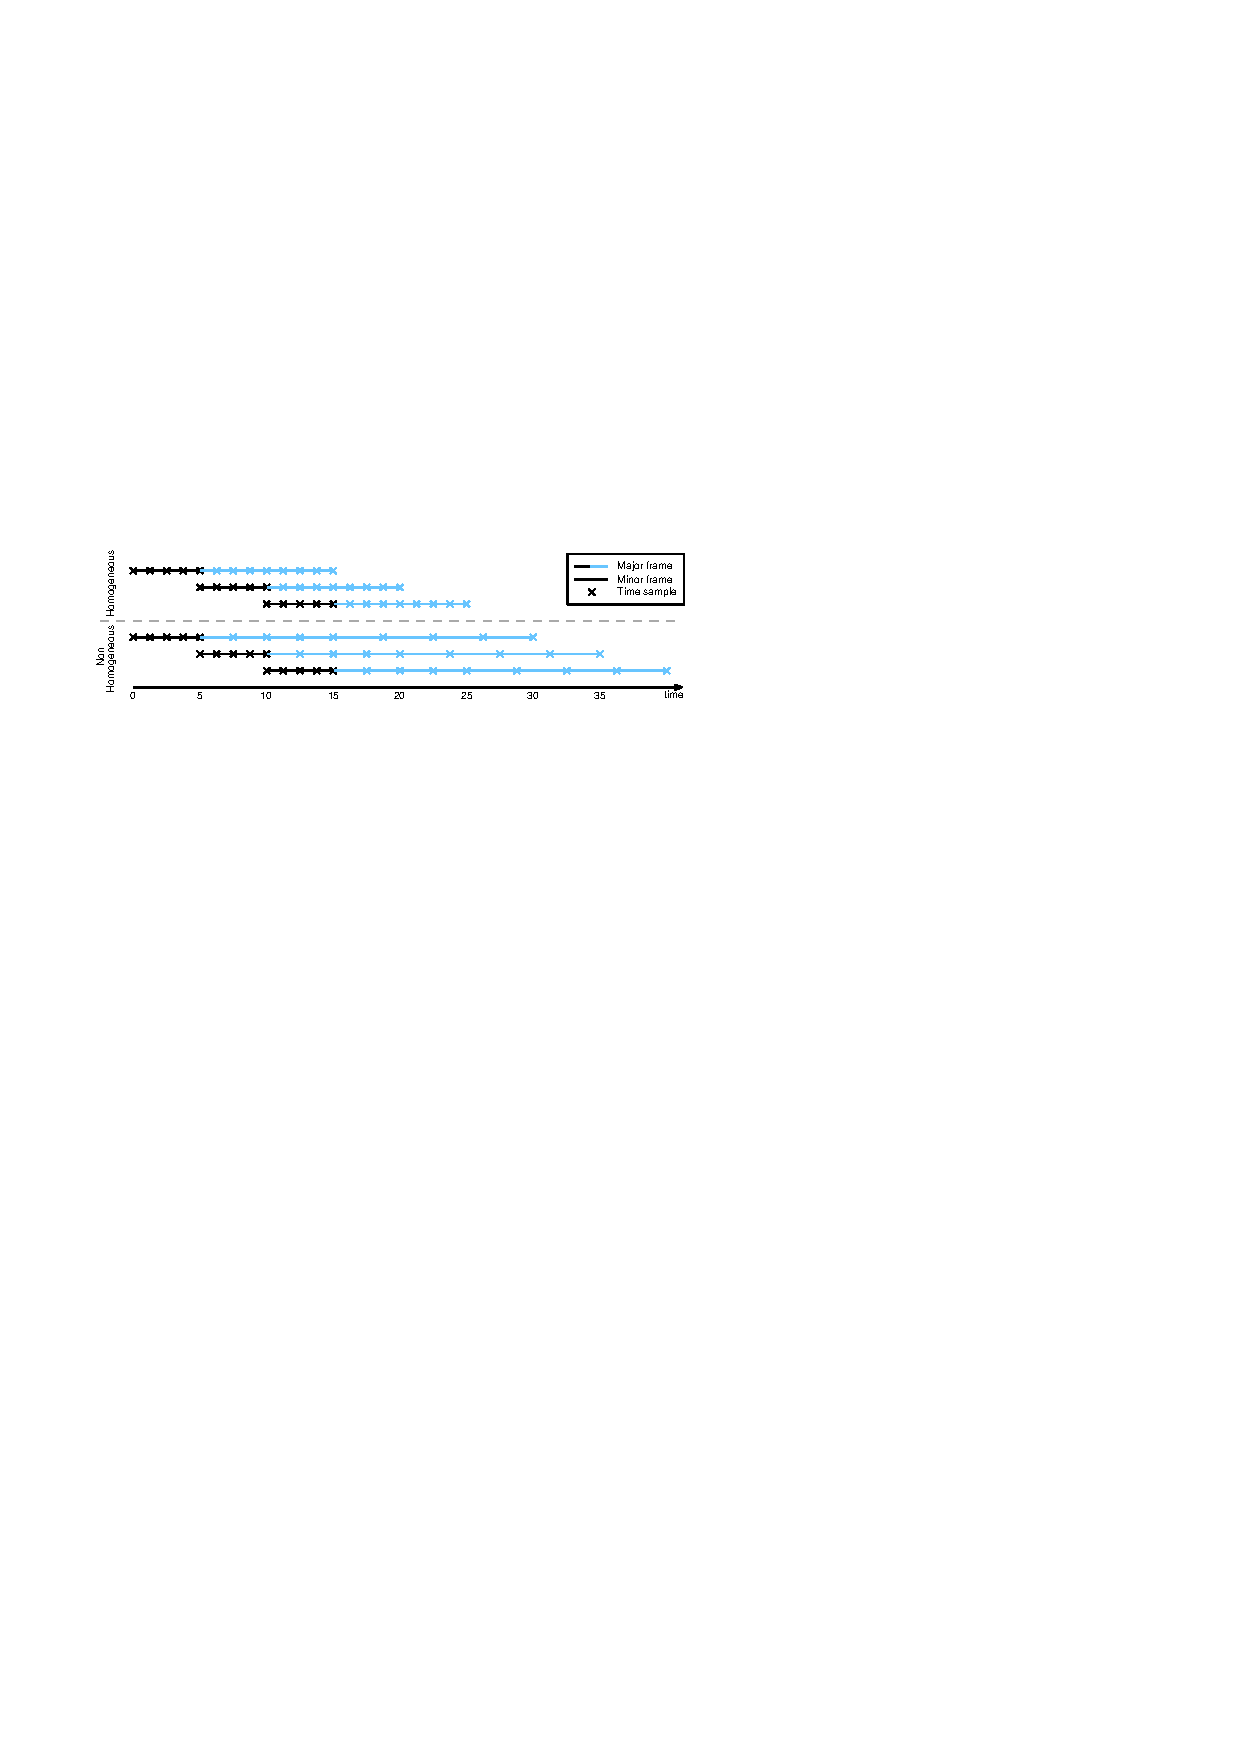
\includegraphics[width=0.75\textwidth]{non_homogeneous_control.png}
\caption{Receding horizon control. In this example, the problem
  horizon \TMAX is 40s. The major frames for MILP optimization are
  discretized in 12 time intervals ($\Nn = 12$) and they span 15s and
  30s for homogeneous and non-homogeneous discretizations,
  respectively.  The minor frames represent the prefix of the 
  major frame MILP optimization that is executed.  The horizon
  recedes by the minor frame duration after each execution.}
\label{fig:multiplan}
\end{figure*}


% def major and minor frame tell about overlapping and fig:multiplan show
% parameters, i.e., delta ts
% - fairness: same delta t for minor frame
For both homogeneous and non-homogeneous intervals, we use the MILP QTM
formulation in a receding horizon manner: a control plan is
computed for a pre-defined horizon (smaller than \TMAX) and only a prefix of
this plan is executed before generating a new control plan. 
%
\cref{fig:multiplan} depicts our receding horizon approach and we refer to the
planning horizon as a major frame and its executable prefix as a minor frame.
%
Notice that, while the plan for a minor frame is being executed, we can start
computing the solution for the next major frame based on a forecast model.


To perform a fair comparison between the homogeneous and non-homogeneous
discretizations, we fix the size of all minor frames to 10s and force it to be
discretized in homogeneous intervals of 0.25s.
%
For the homogeneous experiments, \DT[] is kept at 0.25s throughout the major
frame; therefore, given \Nn, the major frame size equals $\Nn/4$ seconds for the
homogeneous approach.
%
For the non-homogeneous experiments, \DT[] linearly increases from
0.25s at the end of the minor frame to 1.0s at the end of the major frame;
therefore, the major frame size used by the non-homogeneous approach
is $10.375 + 0.625(\Nn-40)$ seconds for a given $\Nn > 40$.
%
%We analyze the effect of the major frame size by varying it from 20s through to 
%120s.
%
% explain evaluation: concatenation + LP simulation Overall ``optimal'' for
% comparison
Once we have generated a series of minor frames, we concatenate them into a
single plan and compute the flow through the network using the QTM LP
formulation with a fixed (homogeneous) $\DT[]$ of 0.25s.
%
%TODO \fnremark{Do we need to justify why we use the QTM as the simulator over
%say a micro simulator?}
%
We also compare both receding horizon approaches against the optimal solution
obtained by computing a single control plan for the entire control horizon
(i.e., $[0,\TMAX]$) using a fixed \DT[] of 0.25s.

\newpage
For all our experiments, we used Gurobi\textsuperscript{TM} as the MILP solver with
12 threads on a 3.1GHz AMD Opteron\textsuperscript{TM}~4334 processor with 12
cores.
%
We limit the MIP gap accuracy to 0.1\% and the time cutoff for solving a major
frame to 3000s for the receding horizon approaches and unbounded in order to
determine the optimal minimum travel time solution to which all other solutions are compared.
%
%% \toIain{Can you explain the following better and provide evidence:
%% \textit{while we can solve non-homogeneous major frames up to convergence in
%% real time, we extend the solve time limit to 3000s for all test points for a
%% fair comparison with the homogeneous test points.}?
%%
%% Iain: Deleted as it was not strictly true. Either we re-run scaled up on AWS
%% with 10s solver time limit. Or we perhaps explain that 3000s shows that it
%% could be scaled up to real time}
%
All our results are averaged over five runs to account for Gurobi's
stochastic strategies.



%\begin{table}[h]
%\caption{Network 3 traffic parameters}
%\label{tab:net3wave}
%\centering
%\begin{tabular}{cccccc}
%\toprule
%Queue & Background & End & Wave & Start &End\\ 
%\midrule
%$q_0$ & 1 & 85 & 1 & 55 & 70\\
%$q_1$ & 2 & 85 & 4 & 55 & 70\\
%$q_4$ & 4 & 85 & 4 & 55 & 70\\
%$q_7$ & 4 & 85 & 4 & 55 & 70\\
%$q_{10}$ & 2 & 85 & 4 & 55 & 70\\
%$q_{14}$ & 4 & 85 & 4 & 55 & 70\\
%$q_{18}$ & 2 & 85 & 4 & 55 & 70\\
%$q_{25}$ & 4 & 85 & 4 & 55 & 70\\
%$q_{29}$ & 2 & 85 & 4 & 55 & 70\\
%$q_{36}$ & 2 & 85 & 4 & 55 & 70\\
%$q_{40}$ & 2 & 85 & 4 & 55 & 70\\
%$q_{44}$ & 2 & 85 & 4 & 55 & 70\\
%\bottomrule\\
%\end{tabular}
%\end{table}


\subsection{Results}


\begin{figure*}[t!]
\centering
%  trim={<left> <lower> <right> <upper>}
\subfigure[]{
\label{subfig:travel_time_3}
\includegraphics[keepaspectratio,height=0.3225\textwidth]{network_1_plot.pdf}}
\subfigure[]{
\label{subfig:delay_3}
\includegraphics[keepaspectratio,height=0.3225\textwidth]{network_1_box_plot.pdf}}
%\includegraphics[keepaspectratio,height=0.3225\textwidth]{box_plot_early_3l.pdf}
%\includegraphics[keepaspectratio,height=0.3225\textwidth]
%{box_plot_converg_3l.pdf}
%\includegraphics[keepaspectratio,height=0.3225\textwidth]{box_plot_final_3l.pdf}}

\subfigure[]{
\label{subfig:travel_time_6}
\includegraphics[keepaspectratio,height=0.3225\textwidth]{network_2_plot.pdf}}
\subfigure[]{
\label{subfig:delay_6}
\includegraphics[keepaspectratio,height=0.3225\textwidth]{network_2_box_plot.pdf}}
%\includegraphics[keepaspectratio,height=0.3225\textwidth]{box_plot_early_6l.pdf}
%\includegraphics[keepaspectratio,height=0.3225\textwidth]
%{box_plot_converg_6l.pdf}
%\includegraphics[keepaspectratio,height=0.3225\textwidth]{box_plot_final_6l.pdf}}

\subfigure[]{
\label{subfig:travel_time_9}
\includegraphics[keepaspectratio,height=0.3225\textwidth]{network_3_plot.pdf}}
\subfigure[]{
\label{subfig:delay_9}
\includegraphics[keepaspectratio,height=0.3225\textwidth]{network_3_box_plot.pdf}}
%\includegraphics[keepaspectratio,height=0.3225\textwidth]{box_plot_early_9l.pdf}
%\includegraphics[keepaspectratio,height=0.3225\textwidth]
%{box_plot_converg_9l.pdf}
%\includegraphics[keepaspectratio,height=0.3225\textwidth]{box_plot_final_9l.pdf}}
%
\caption{Increase in the total travel time w.r.t.~the optimal solution as a
function of \Nn (a,c,e) and distribution of the total delay of
each car for different values of \Nn (b,d,f).
%
For each row, the Roman numeral on top of the box plots corresponds to points on the 
travel time plot marked with the same numeral.
%
The mean of the total delay is presented as a red square in the box plots.
%
Plots in the $i$-th row correspond to the results for the $i$-th network in
\cref{fig:networks}.  Non-homogeneous (NH) achieves much better solutions
at smaller \Nn than Homogeneous (H).}
%control and achieves }
%smaller third quartile and maximum per-car delay for the same \Nn.}
\label{fig:results}
\end{figure*}


%We compare the performance of non-homogeneous and homogeneous solutions in two
%ways: comparing the decrease in total travel time with increasing major frame
%time (greater look ahead), and analysing the distribution of delay in each
%queue of the network.
%
\cref{subfig:travel_time_3,subfig:travel_time_6,subfig:travel_time_9} show, for
each network, the increase in the total travel time w.r.t.~the optimal solution
as a function of \Nn.
%
As we hypothesized, the non-homogeneous discretization requires less time
intervals (i.e., smaller \Nn) to obtain a solution with the same total travel
time.
%
This is important because the size of the MILP, including the number of binary
variables, scales linearly with \Nn; therefore, the non-homogeneous approach can
scale up better than the homogeneous one (e.g., \cref{subfig:travel_time_9}).
%
Also, for homogeneous and non-homogeneous discretizations, finding the optimal
solution of major frames with large \Nn might require more time than our imposed
3000s time cutoff and, in this case, Gurobi returns a feasible control plan that
is far from optimal.
%
The effect in the total travel time of these poor solutions can be seen in
\cref{subfig:travel_time_9} for $\Nn > 120$.



The distribution of the total delay observed by each car while traversing the
network is shown in \cref{subfig:delay_3,subfig:delay_6,subfig:delay_9}.
%
Each group of box plots represents a different value of~\Nn: when the
non-homogeneous $\DT[]$ first converges; when the homogeneous~$\DT[]$ first
converges; and the optimum solution itself.
%
In all networks, the quality of the solution obtained using non-homogeneous
$\DT[]$ is better or equal than using homogeneous $\DT[]$ for fixed \Nn in both
the total travel time and \emph{fairness}, i.e., smaller third quartile and
maximum delay.

%\remark{FWT: In the paragraphs above, we need to address network 2 because it is
%the exception in both cases: in the end of \cref{subfig:travel_time_6},
%homogeneous is better, and the homogeneous delay in \cref{subfig:delay_6} is
%also better.}


\begin{figure*}[t!]
\centering

%  trim={<left> <lower> <right> <upper>}
\subfigure[]{
\label{subfig:cumu1}
\includegraphics[width=0.32\textwidth]{network_2_cum_plot_early.pdf}}
\subfigure[]{
\label{subfig:cumu2}
\includegraphics[width=0.32\textwidth]{network_2_cum_plot_converg.pdf}}
\subfigure[]{
\label{subfig:cumu3}
\includegraphics[width=0.32\textwidth]{network_2_cum_plot_final.pdf}}
%
\caption{Cumulative arrival and departure curves and delay for queue 1 in the
2-by-3 network (\cref{subfig:network2}).
%
The labels on top of each plot match the labels in
\cref{subfig:travel_time_6,subfig:delay_6}.
%
(c)~presents the same curves for the optimal solution.  Non-homogeneous~(NH)
provides near-optimal signal plans over a longer time horizon than
Homogeneous~(H) when the number of time intervals \Nn is small.}
%
\label{fig:cumu}
\end{figure*}


To further illustrate the differences between homogeneous and non-homogeneous
discretizations, \cref{fig:cumu} shows the cumulative arrival and departure
curves and the how delay evolves over time for $q_1$ of network 2
(\cref{subfig:network2}).
%
In \cref{subfig:cumu1}, the comparison is done when non-homogeneous $\DT[]$
first converges (i.e., point I in \cref{subfig:travel_time_6}) and for this
value of \Nn, the major frame size in seconds of the non-homogeneous approach is
19.125s longer than the homogeneous one.
%
This allows the MILP solver to ``see'' 19s further in the future when using
non-homogeneous discretization and find a coordinated signal policy along the
avenue to dissipate the extra traffic that arrives at time 55s.
%
The shorter major frame of the homogeneous discretization does not allow the
solver to adapt this far in advance and its delay observed after 55s is much
larger than the non-homogeneous one.
%
Once the homogeneous $\DT[]$ has converged (\cref{subfig:cumu2}), it is also
able to anticipate the increased demand and adapt well in advance and both
approaches generate solutions close to optimum (\cref{subfig:cumu3}).


\section{Conclusion}

In this paper, we studied how to mitigate the impact of light rail on
conventional traffic networks via a novel method of optimized traffic
signal control based on Mixed Integer Linear Programming (MILP). Our
key results show that while there is a substantial impact of light
rail on conventional vehicle traffic delay using popular fixed-time
signal control, our novel optimized signal control virtually nullifies
this impact. Ultimately this leads to a win-win situation where both
conventional vehicle traffic and light rail commuters benefit through
the application of MILP-based optimization.

\Omit{
In this paper, we showed how to formulate a novel queue transmission model (QTM)
model of traffic flow with non-homogeneous time steps as a linear program.  We
then proceeded to allow the traffic signals to become discrete variables subject
to a delay minimizing optimization objective and standard traffic signal
constraints leading to a final MILP formulation of traffic signal control with
non-homogeneous time steps.  We
experimented with this novel QTM-based MILP control in a range of traffic networks
and demonstrated that the non-homogeneous MILP formulation
achieved (i) substantially lower delay solutions, (ii) improved per-car delay distributions,
and (iii) more optimal travel times over a longer horizon 
in comparison to the homogeneous MILP formulation with the same number of binary
and continuous variables.
%% NOTE: what bothers me here is ``larger networks'' since we don't directly
%%       compare scalability of the approaches as a function of network size
%%       (i.e., on the x-axis of some graph).  -Scott
%and demonstrated that by exploiting the non-homogeneous time steps supported
%by the QTM, we are able to scale the model up to larger networks whilst maintaining the
%same quality of a homogeneous solution using more binary
%variables.
Altogether, this work represents a
major step forward in the scalability of MILP-based jointly optimized traffic
signal control via the use of a non-homogeneous time traffic models and thus helps
pave the way for fully optimized joint urban traffic signal controllers as an
improved successor technology to existing signal control methods.
}

%We have demonstrated that by exploiting the non-homogeneous time steps
%supported by the QTM, we are able to scale the model up to larger
%networks and using the same number of binary variables as a
%homogeneous time step, and with the same quality of a homogeneous
%solution using more binary variables.


\bibliographystyle{trb}
\bibliography{Transport}

% End line numbering
\nolinenumbers
\end{document}
